% CVPR 2023 Paper Template
% based on the CVPR template provided by Ming-Ming Cheng (https://github.com/MCG-NKU/CVPR_Template)
% modified and extended by Stefan Roth (stefan.roth@NOSPAMtu-darmstadt.de)

\documentclass[10pt,twocolumn,letterpaper]{article}

%%%%%%%%% PAPER TYPE  - PLEASE UPDATE FOR FINAL VERSION
\usepackage[review]{cvpr}      % To produce the REVIEW version
%\usepackage{cvpr}              % To produce the CAMERA-READY version
%\usepackage[pagenumbers]{cvpr} % To force page numbers, e.g. for an arXiv version

% Include other packages here, before hyperref.
\usepackage{graphicx}
\usepackage{amsmath}
\usepackage{amssymb}
\usepackage{booktabs}
\usepackage{bm}


% It is strongly recommended to use hyperref, especially for the review version.
% hyperref with option pagebackref eases the reviewers' job.
% Please disable hyperref *only* if you encounter grave issues, e.g. with the
% file validation for the camera-ready version.
%
% If you comment hyperref and then uncomment it, you should delete
% ReviewTempalte.aux before re-running LaTeX.
% (Or just hit 'q' on the first LaTeX run, let it finish, and you
%  should be clear).
\usepackage[pagebackref,breaklinks,colorlinks]{hyperref}


% Support for easy cross-referencing
\usepackage[capitalize]{cleveref}
\crefname{section}{Sec.}{Secs.}
\Crefname{section}{Section}{Sections}
\Crefname{table}{Table}{Tables}
\crefname{table}{Tab.}{Tabs.}


%%%%%%%%% PAPER ID  - PLEASE UPDATE
\def\cvprPaperID{*****} % *** Enter the CVPR Paper ID here
\def\confName{CVPR}
\def\confYear{2023}


\begin{document}

%%%%%%%%% TITLE - PLEASE UPDATE
\title{PRFDN: Reparameterize and Prune Disentangled U-Net for Efficient Image Super-resolution}
%多路径

\author{Daheng Yin, Baijun Chen, Mengyang Liu, Fang Dong\\
School of Computer Science and Engineering, Southeast University, Nanjing, China\\
{\tt\small \{yindaheng98, bjchen, myliu, fdong\}@seu.edu.cn}
}
\maketitle

%%%%%%%%% ABSTRACT
\begin{abstract}
  Single image super-resolution (SISR) is a computer vision technique that uses deep convolution neural networks to reconstruct high-resolution images from low-resolution images. It has been used in many applications, but due to power constraints on mobile devices, efficient image super-resolution (EISR) is becoming increasingly important and researchers are designing lightweight networks through methods like network pruning, parallelism, and knowledge distillation.
  Efficient network design is key to achieving better performance in EISR, and many designs adopt the U-Net architecture. By deconstructing its branching structure, the main structure of the U-Net can be transformed into mutually independent branches, increasing parallelism and reducing the number of layers executed serially in the network to improve inference speed within the GPU's capacity.
  This paper proposed Parallel RFDN (PRFDN) based on the pre-trained RFDN, which is a typical EISR model with a backbone similar to U-Net. 
  Our method disentangles the sequentially computed trunks in RFDN into branches and performs re-parametrization to make these branches inference in parallel on single devices. 
  After that, we further perform pruning on the model and finetune it to achieve higher performance.
  %TODO: 补充一句实验结果
\end{abstract}

%%%%%%%%% BODY TEXT
\section{Introduction}
\label{sec:intro}

Single image super-resolution (SISR) is a computer vision technique to reconstruct high-resolution images from low-resolution images. Deep convolution neural networks have shown impressive performance in this area and many deep learning-based methods have been proposed to address this ill-posed problem.
This technique has been used in many applications (e.g. video gaming\cite{10.1145/2751496.2751502} and video streaming\cite{kimNeuralEnhancedLiveStreaming2020,yeoNeuralAdaptiveContentaware2018,maoNeuralAdaptiveVideo2017}) to achieve displays with high resolution and high refresh rates and some of the related applications have been deployed on lots of mobile devices\cite{yeoNEMOEnablingNeuralenhanced2020,mehtaEVRNetEfficientVideo2021}.
However, mobile phones have a power-constrained design with a dedicated power supply, which makes efficient image super-resolution (EISR) a growing interest.

Efficient network design is key to achieving better performance in EISR.
To make the network more efficient for resource-limited devices, researchers are designing generic lightweight networks with reduced parameters through methods like network pruning\cite{liuSplitSREndtoEndApproach2021,leeMobiSREfficientOnDevice2019,fang2023depgraph}, parallelism\cite{sandlerMobileNetV2InvertedResiduals2019,howardMobileNetsEfficientConvolutional2017,liuSplitSREndtoEndApproach2021,kongClassSRGeneralFramework2021} and knowledge distillation\cite{liu2020residual,khaniRealTimeVideoInference2021,taoCompressionGenerativePretrained2022,zhangDataFreeKnowledgeDistillation2021}.
However, when the model size becomes sufficiently small, these methods fail to further increase the frame rate of super-resolution. This is because reducing the computational scale of each layer of the model beyond the point where the GPU is fully loaded does not improve the inference speed of the model, if the length of serially executed layers cannot be reduced.
Therefore, lots of EISR designs\cite{liNTIRE2022Challenge2022,duFastMemoryEfficientNetwork2022,mehtaEVRNetEfficientVideo2021} involve careful consideration of network architecture, design, and utilization of limited features to generate more representative features for super-resolution, which can use fewer layers to achieve a good super-resolution quality.

Moreover, recent years have witnessed the wide use of U-Net\cite{ronnebergerUNetConvolutionalNetworks2015} in the design of deep neural networks. 
Many designs of the EISR model also adopted the U-Net architecture, and the RFDN\cite{liu2020residual} is a representative example, which won the first prize in the AIM 2020 competition. 
Through the observation of the U-Net structure, we found its main structure can be transformed into mutually independent branches by deconstructing its branching structure, thereby increasing parallelism. 
Furthermore, multiple branches can be executed in parallel on the same GPU by reparameterization. 
Within the GPU's capacity, this method can reduce the number of layers that are executed serially in the network, therefore improving the inference speed.

In this paper, we proposed Parallel RFDN (PRFDN) based on the pre-trained RFDN. Our method disentangles the sequentially computed trunks in RFDN into branches and performs re-parametrization to make these branches inference in parallel on single devices. After that, we further perform pruning on the model and finetune it to achieve higher performance.

\subsection{Paper ID}
Make sure that the Paper ID from the submission system is visible in the version submitted for review (replacing the ``*****'' you see in this document).
If you are using the \LaTeX\ template, \textbf{make sure to update paper ID in the appropriate place in the tex file}.


\subsection{Methods}

We proposed Parallel RFDN (PRFDN) as is shown in figure \ref{fig:PRFDN}.
Our method consists of four stages to transform a pre-trained RFDN\cite{liu2020residual} into PRFDN.

\subsection{Branching}
To accelerate the inference, we first consider reducing the data dependency in the model to achieve higher parallelism. 
According to our observation, the main structure of U-Net can be transformed into mutually independent branches to increase parallelism. 
Our method disentangles the sequentially computed trunks of RFDN into branches. 
As is shown in figure \ref{fig:Branching}, after the branching, the major part of the model will consist of four independent branches that can calculate in parallel. 
To improve the accuracy, we also design a small SR block (SRFDB) based on the RFDB of RFDN and add them before the input of each branch. 
% This type of block 用于拟合多层RFDB的输出结果,使得输入到被展开后的RFDB block的输入与其在原始模型中接收的输入相近,从而以一个较小的代价保证模型精度
This type of block is utilized to fit the output of cascaded RFDBs, such that the input to the disentangled RFDB block closely resembles the input received in the original RFDN.
This ensures model accuracy at a reduced cost.

\subsection{Training}
Since we only change the data flow but not the structure of RFDB, the pre-trained RFDN parameters can still be loaded into the major part of our branch model (only except for those SRFDBs). 
To benefit from the pre-training, we load the pre-trained RFDN parameters into our branch model before training our branch model.
In this step, we first trained only SRFDBs for 100 epochs (on LSDIR dataset and DIV2K dataset) with freeze parameters in RFDBs, and then trained the whole model for 100 epochs.

\subsection{Re-parametrization}
Without much data dependency, branches in our model can be computed in parallel. 
However, a single GPU cannot compute two or more different models in parallel. 
To address this issue and achieve parallel computing of multiple branches on a single GPU, we should merge the four branches into a single branch. 
As is shown in figure \ref{fig:Branching}, three of these four branches have exactly the same structure with only different parameters, and the only difference between the remaining branch and the other branches is the absence of an RFDBS.
Therefore, we should 1) merge those four convolution layers at the beginning of the branches into one, 2) merge those three RFDBS into one, and 3) merge those four RFDBs into one.

In our method, we create a bigger RFDB and a bigger SRFDB with bigger convolution layers and move the weight and bias from the RFDBs and SRFDBs into them.
More specifically, we merge the convolution layers according to the following derivation.

Assuming $Y=Conv(X, K)$ represents a convolution layer,
where $K\in\mathbb{R}^{c_o\times c\times h_k\times w_k}$ is the convolution kernel; $X\in\mathbb{R}^{c\times h\times w}$ is the input of convolution layer and $Y\in\mathbb{R}^{c_o\times h'\times w'}$ is the output; 
$c$, $h$, $w$ are the channel, height, and width of the input respectively; 
$c_o$, $h'$, $w'$ are the channel, height, and width of the output respectively;
$h_k$ and $w_k$ are the height and width of the kernel respectively.
If we want to merge $n$ convolution layers $Y_i=Conv(X_i, K_i)$ into a big convolution layer $Conv_b$, this $Conv_b$ can be represented as:
\begin{equation}
  \begin{aligned}
    Y&=Conv_b([X_1,\dots,X_n], K_1,\dots,K_n)\\
    &=[Y_1,\dots,Y_n]\\
    &=\sum_{i=1}^n[\bm 0,\dots,Y_i,\dots,\bm 0]\\
    &=\sum_{i=1}^n[\bm 0,\dots,Conv(X_i, K_i),\dots,\bm 0]\\
    &=Conv([X_1,\dots,X_n], 
    \begin{bmatrix}
      K_1 & \bm 0 & \dots & \bm 0 \\
      \bm 0 & K_2 & \dots & \bm 0 \\
      \vdots & \vdots & \ddots & \vdots \\
      \bm 0 & \bm 0 & \dots & K_n \\
    \end{bmatrix})\\
    &=Conv(X_{concat}, K_{diag})
  \end{aligned}
\end{equation}

Therefore, when computing the merged convolution layer $Conv_b$, all the input $X_i, i\in[1,n]$ would be concatenated into $X_{concat}$ and all the kernel $K_i, i\in[1,n]$ would be re-parameterized into $K_{diag}$ (in first two dimensions) before performing a normal convolution operation.

Inspired by Torch-Pruning\cite{fang2023depgraph}, we implemented our re-parametrization algorithm as a convolution constructor function:
\begin{verbatim}
def merge_conv(convs, c, c_o, k, **kwargs):
  n = len(convs)
  conv = nn.Conv2d(c*n, c_o*n, k, **kwargs)
  for i, j in product(range(n), range(n)):
    if j == i:
      conv.weight[j*c_o:(j+1)*c_o,
                  i*c:(i+1)*c,
                  ...] = \
        convs[i].weight
    else:
      conv.weight[j*c_o:(j+1)*c_o,
                  i*c:(i+1)*c,
                  ...] = \
        torch.zeros(convs[i].weight.shape)
  for i in range(n):
      conv.bias[i*c_o:(i+1)*c_o] = \
        convs[i].bias
  return conv
\end{verbatim}

As is shown in figure \ref{fig:Re-parametrization}, we merge and re-parametrize the four convolution layer, three SRFDBs and four RFDBs into a bigger convolution layer, SRFDB and RFDB respectively. 
After re-parameterization, we get a bigger model that is equivalent to that of the branches of the branch model computed in parallel on a single GPU.

\subsection{Pruning}
The re-parametrized model is big. To reduce the resource consumption and further accelerate the inference, we applied selective channel-wise auto-pruning (Torch-Pruning\cite{fang2023depgraph}) on our re-parametrized model, as is shown in figure \ref{fig:Pruning}. 

Specifically, as channel-wise pruning would modify the output channel number of certain layers (especially convolution layers), channel indices of channel-wise split and concatenate operations should be adjusted accordingly.
However, determining which channels are pruned during auto-pruning is difficult to implement in code.
In our method, we propose to replace all channel-wise split and concatenate operations with equivalent 1x1 convolutions.
This allows auto-pruning to directly prune these operations and eliminates the need to adjust their channel indices separately.

After re-parametrization, we used Torch-Pruning to prune the model.
In our implementation, we prune out 90\% channels from our model in 16 steps, and between each pruning step, we finetune the model by a 10-epoch training.

\begin{figure*}
    \centering
    \begin{subfigure}[b]{0.49\linewidth}
		\centering
        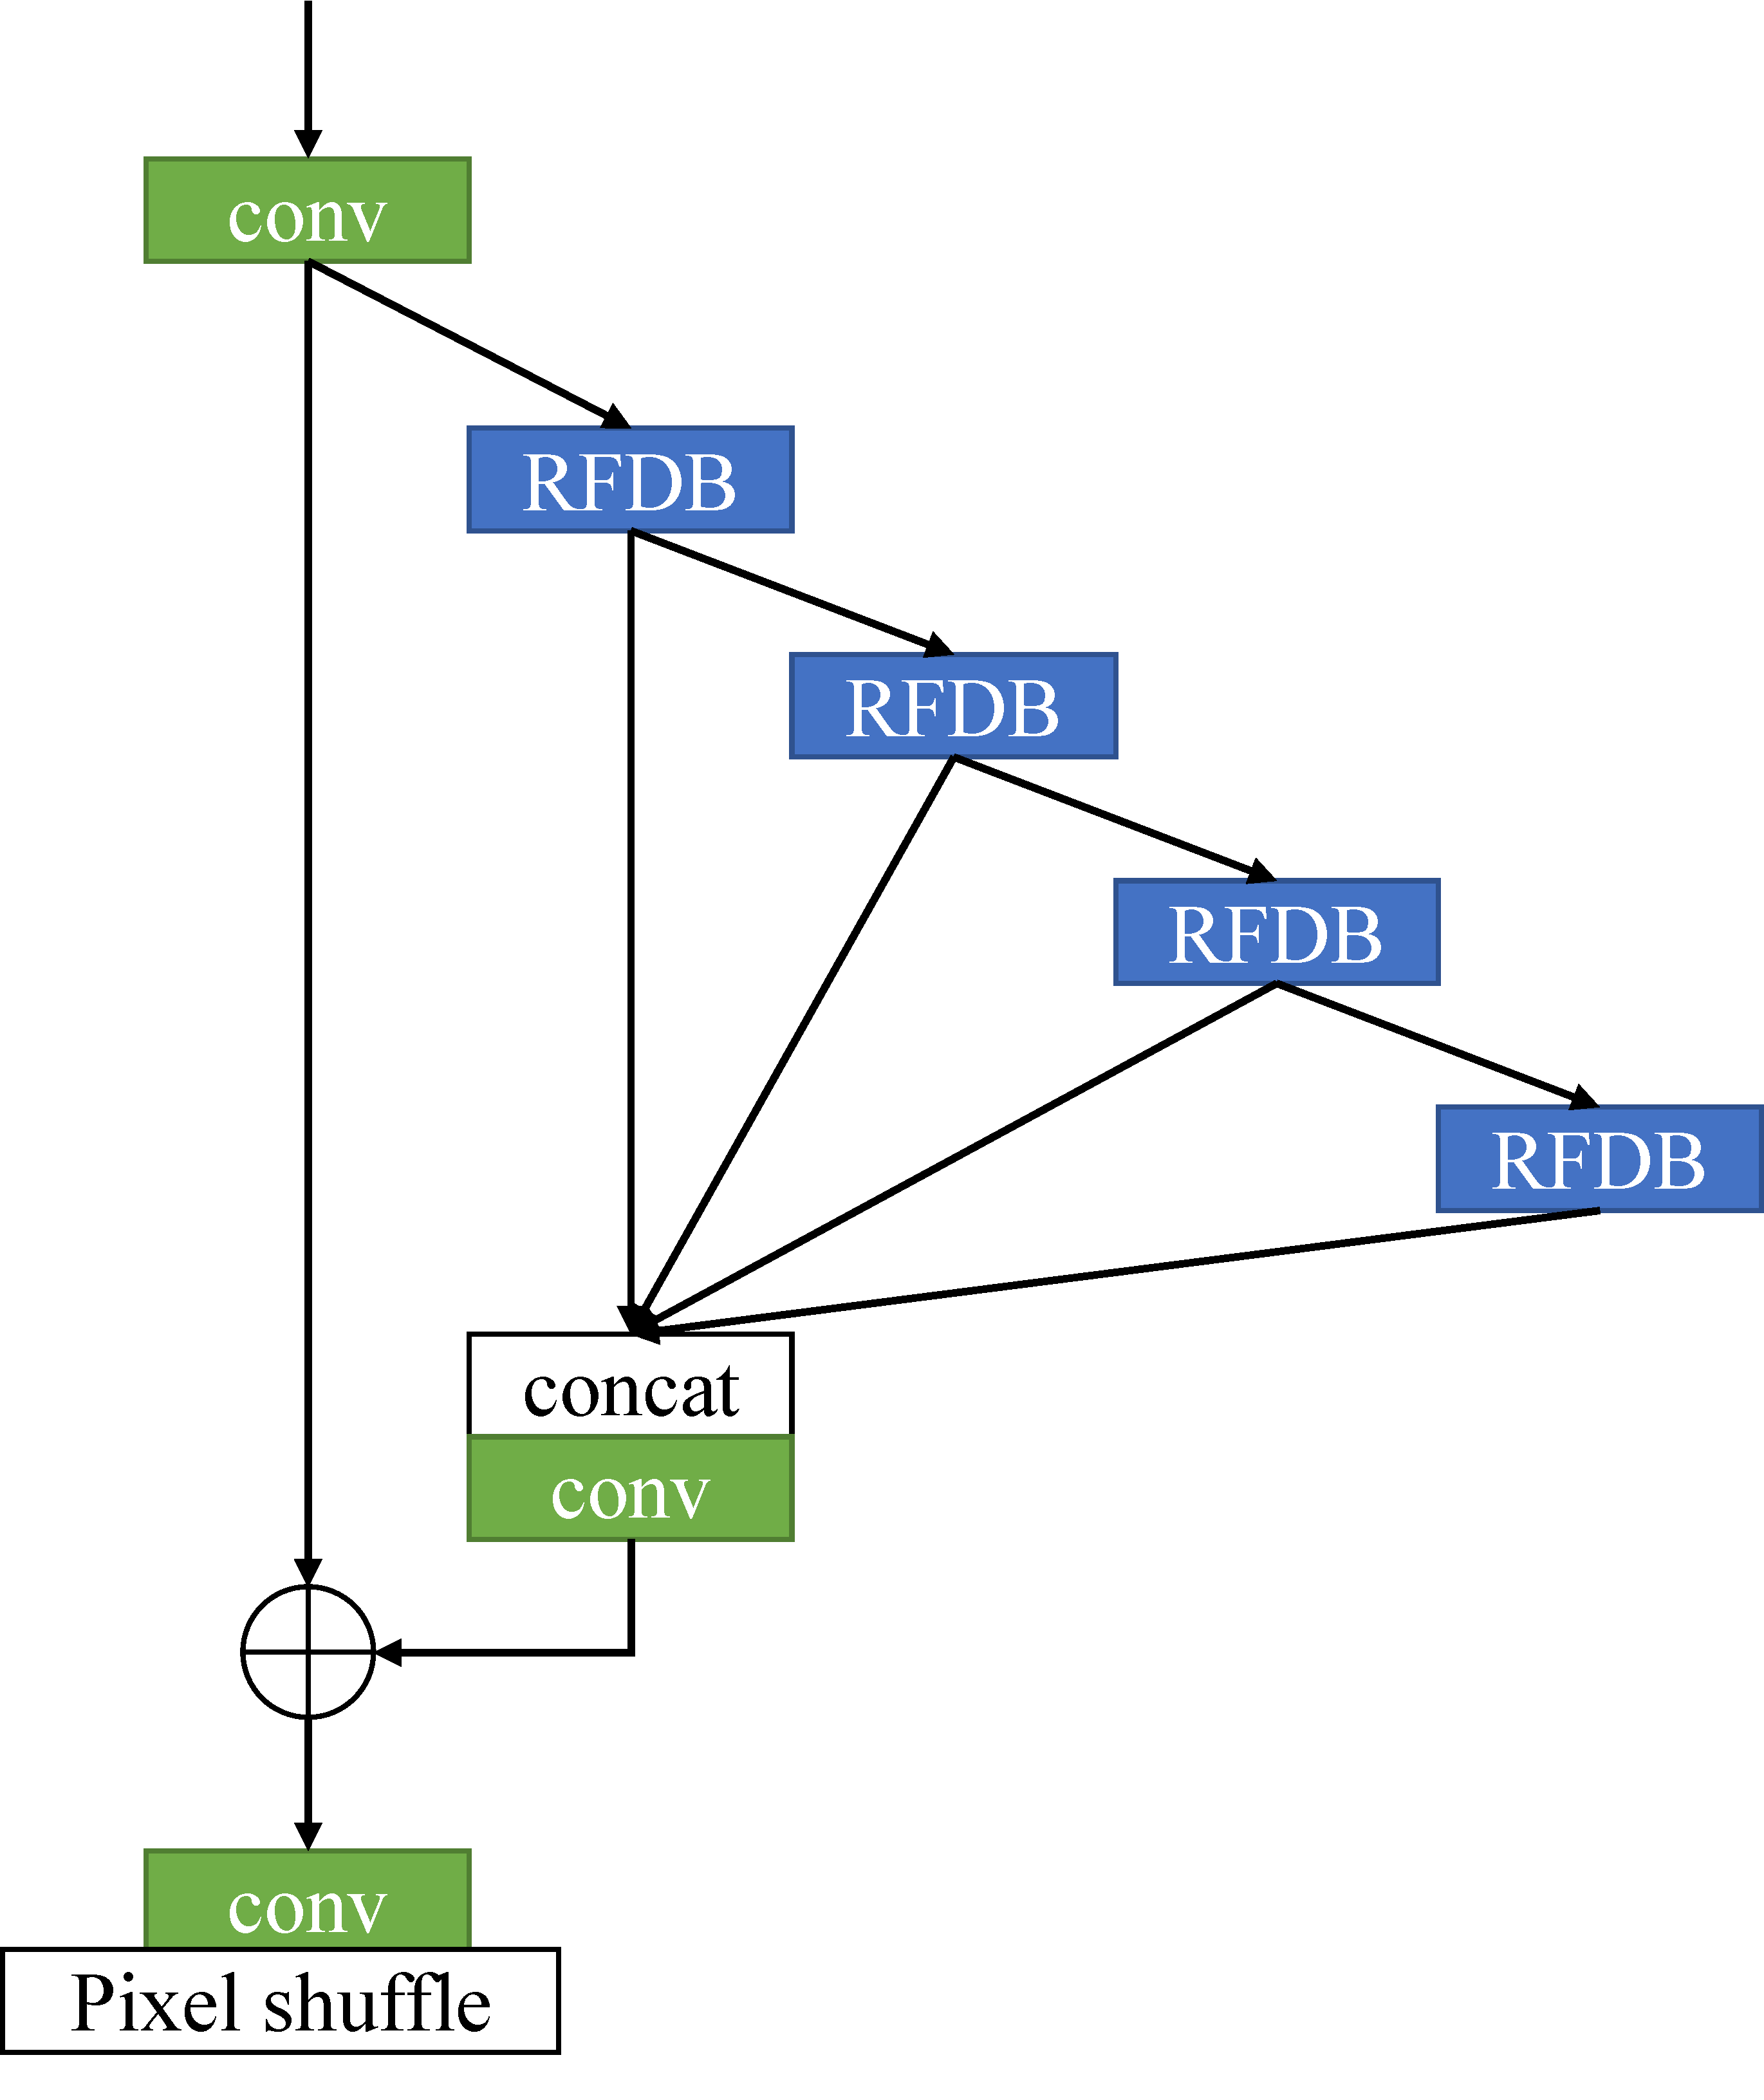
\includegraphics[width=\textwidth]{../RFDN.pdf}
        \caption{RFDN}
        \label{fig:RFDN}
    \end{subfigure}
    \begin{subfigure}[b]{0.49\linewidth}
		\centering
        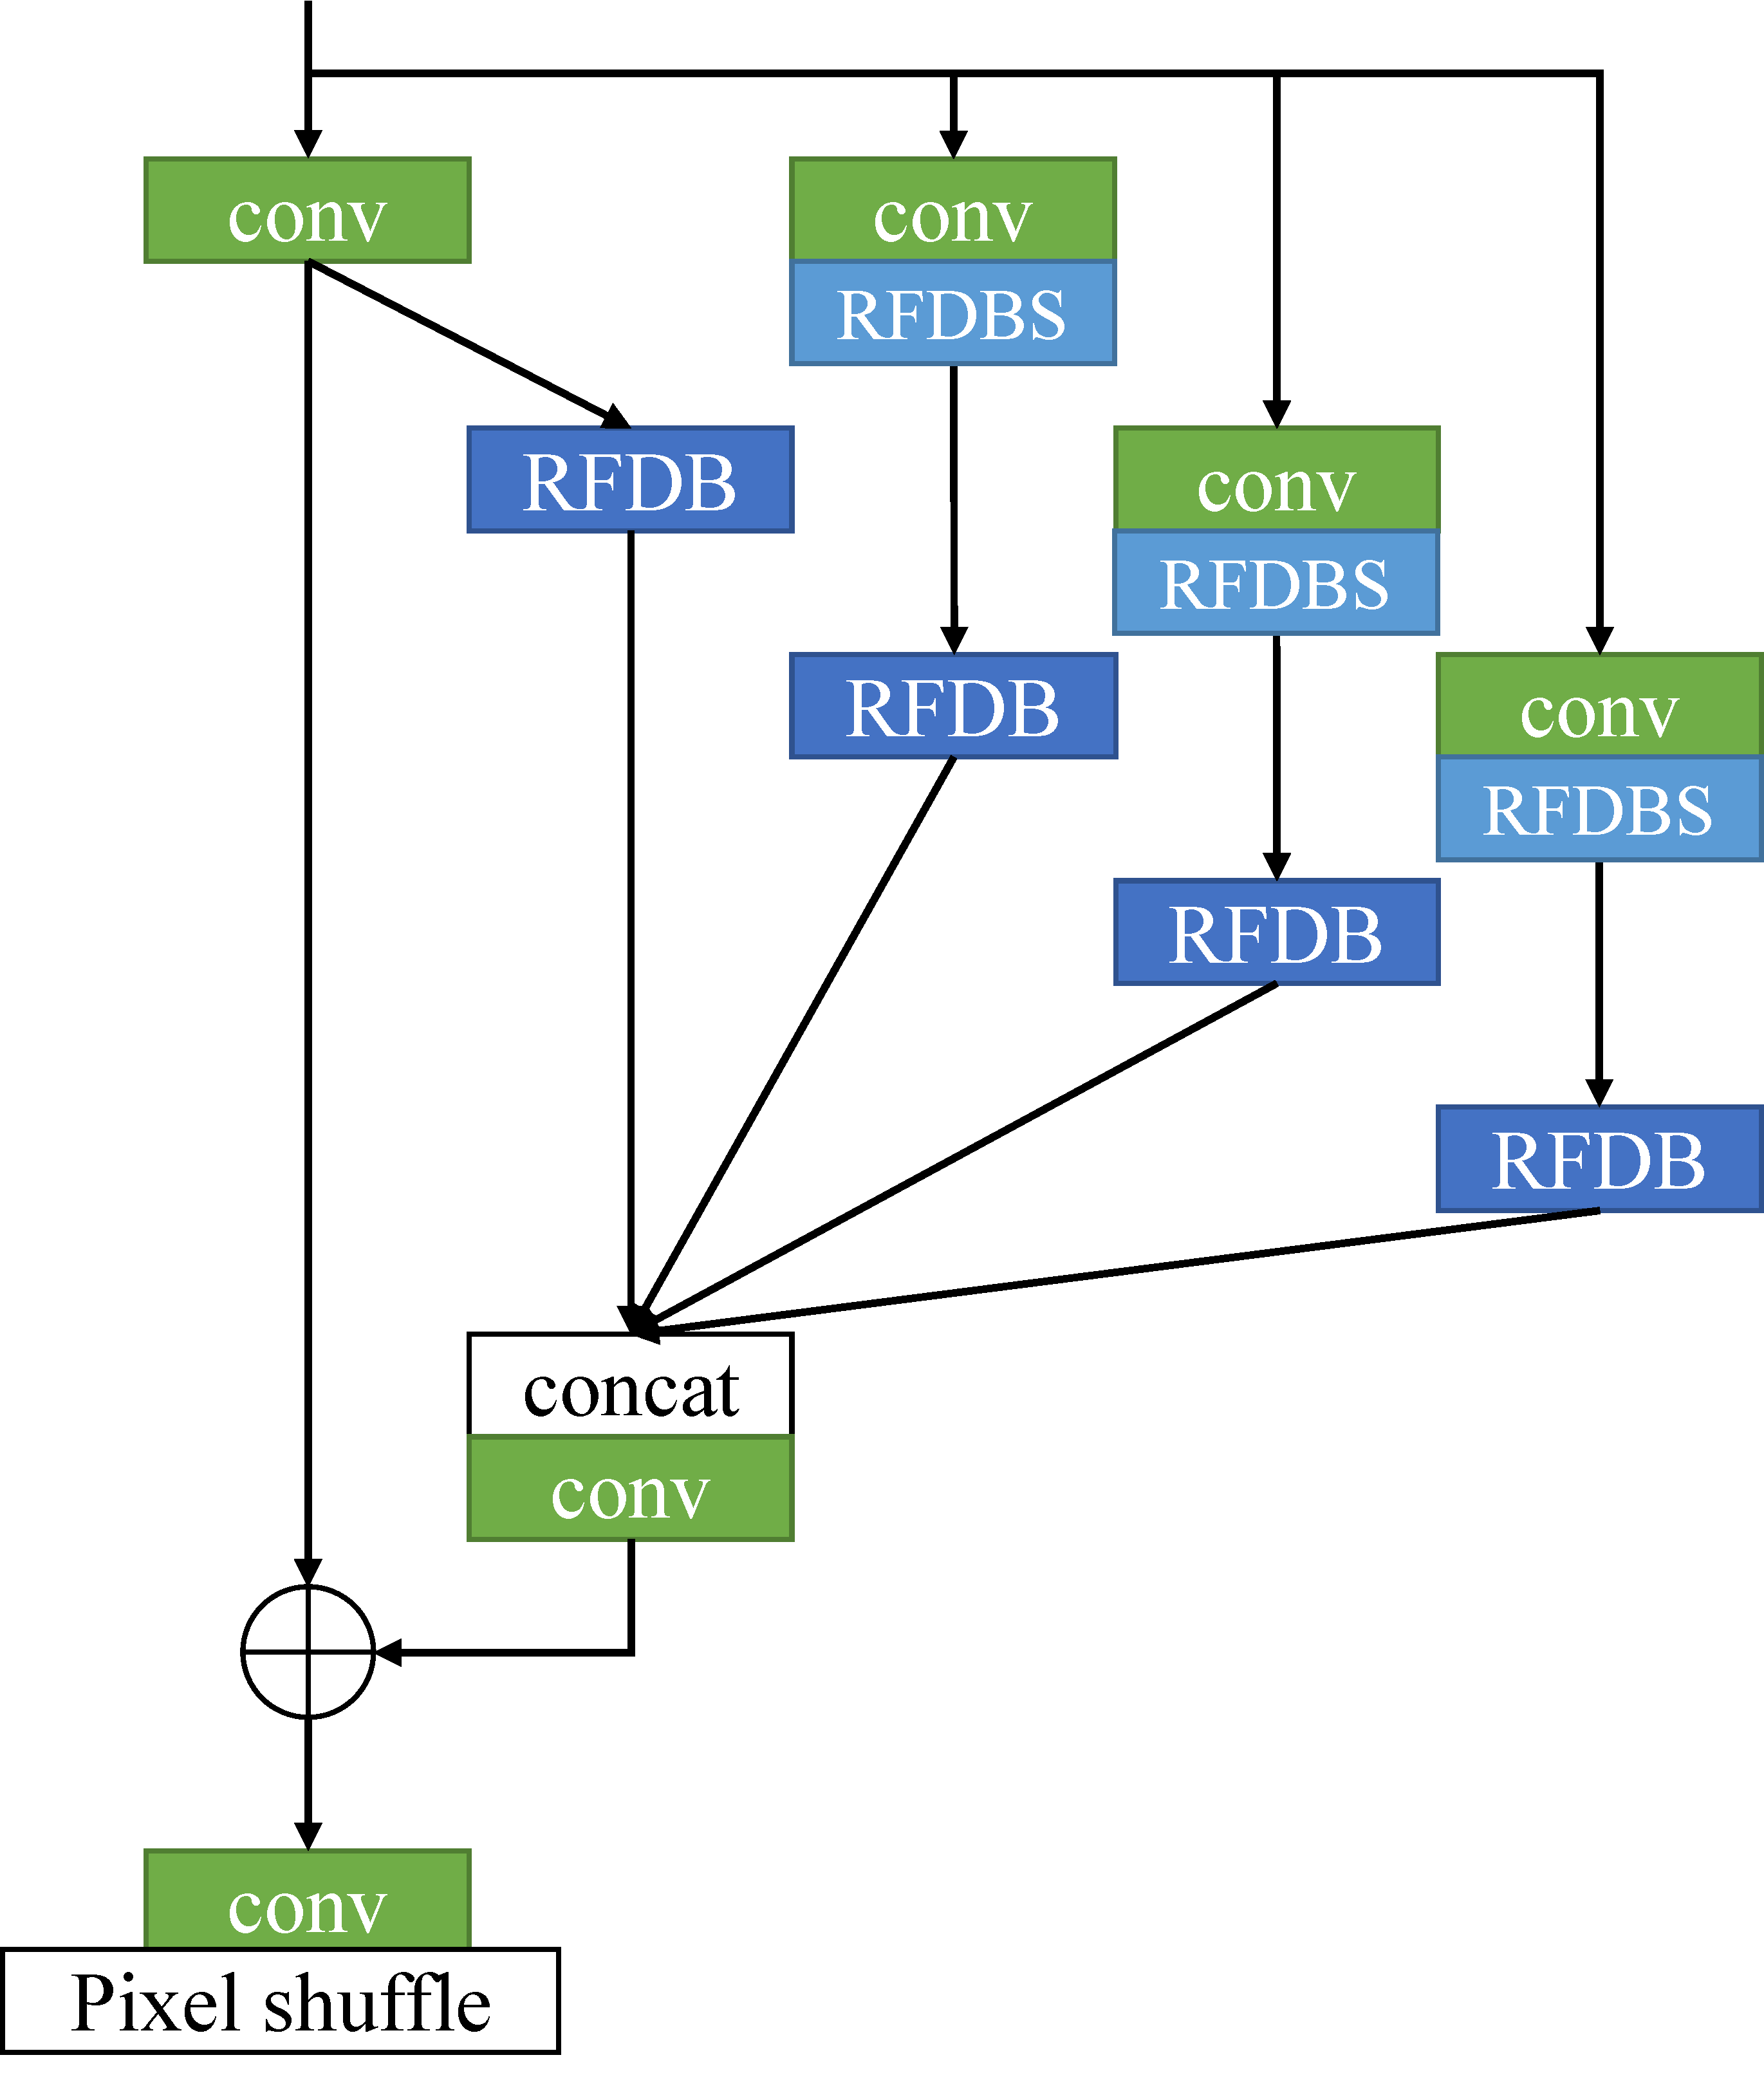
\includegraphics[width=\textwidth]{../Branching.pdf}
        \caption{Branching}
        \label{fig:Branching}
    \end{subfigure}
    \begin{subfigure}[b]{0.49\linewidth}
		\centering
        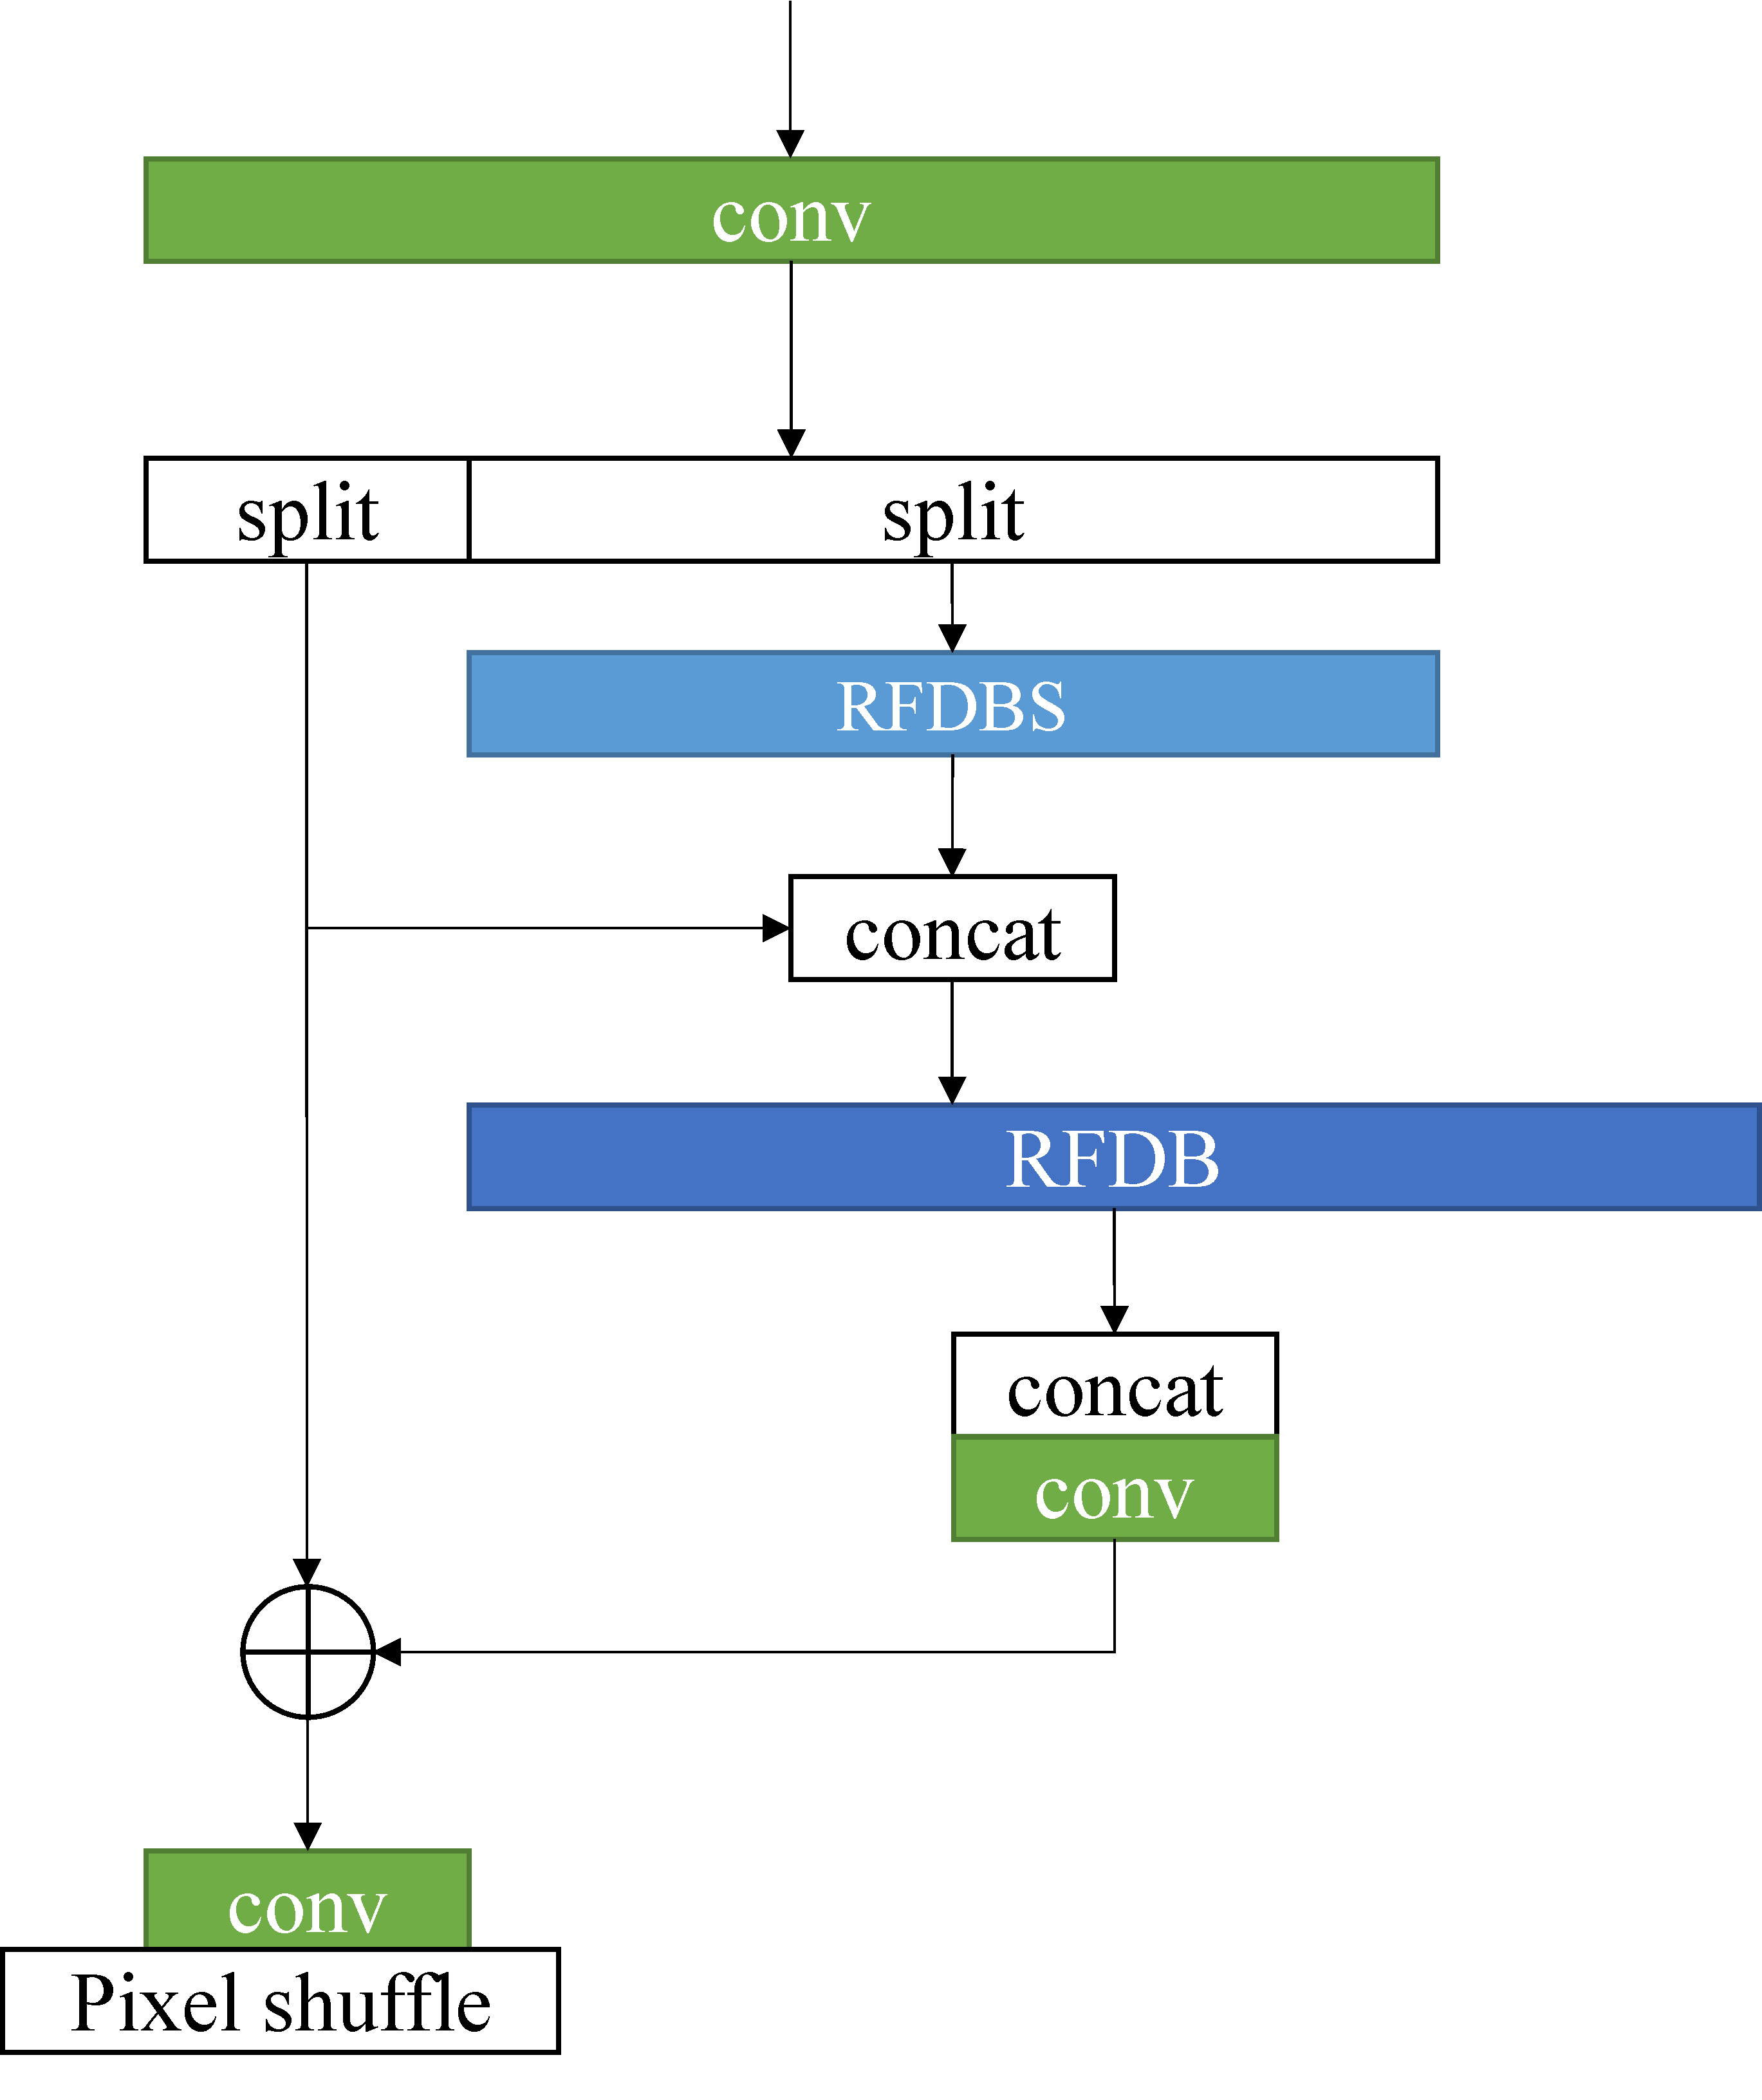
\includegraphics[width=\textwidth]{../Re-parametrization.pdf}
        \caption{Re-parametrization}
        \label{fig:Re-parametrization}
    \end{subfigure}
    \begin{subfigure}[b]{0.49\linewidth}
		\centering
        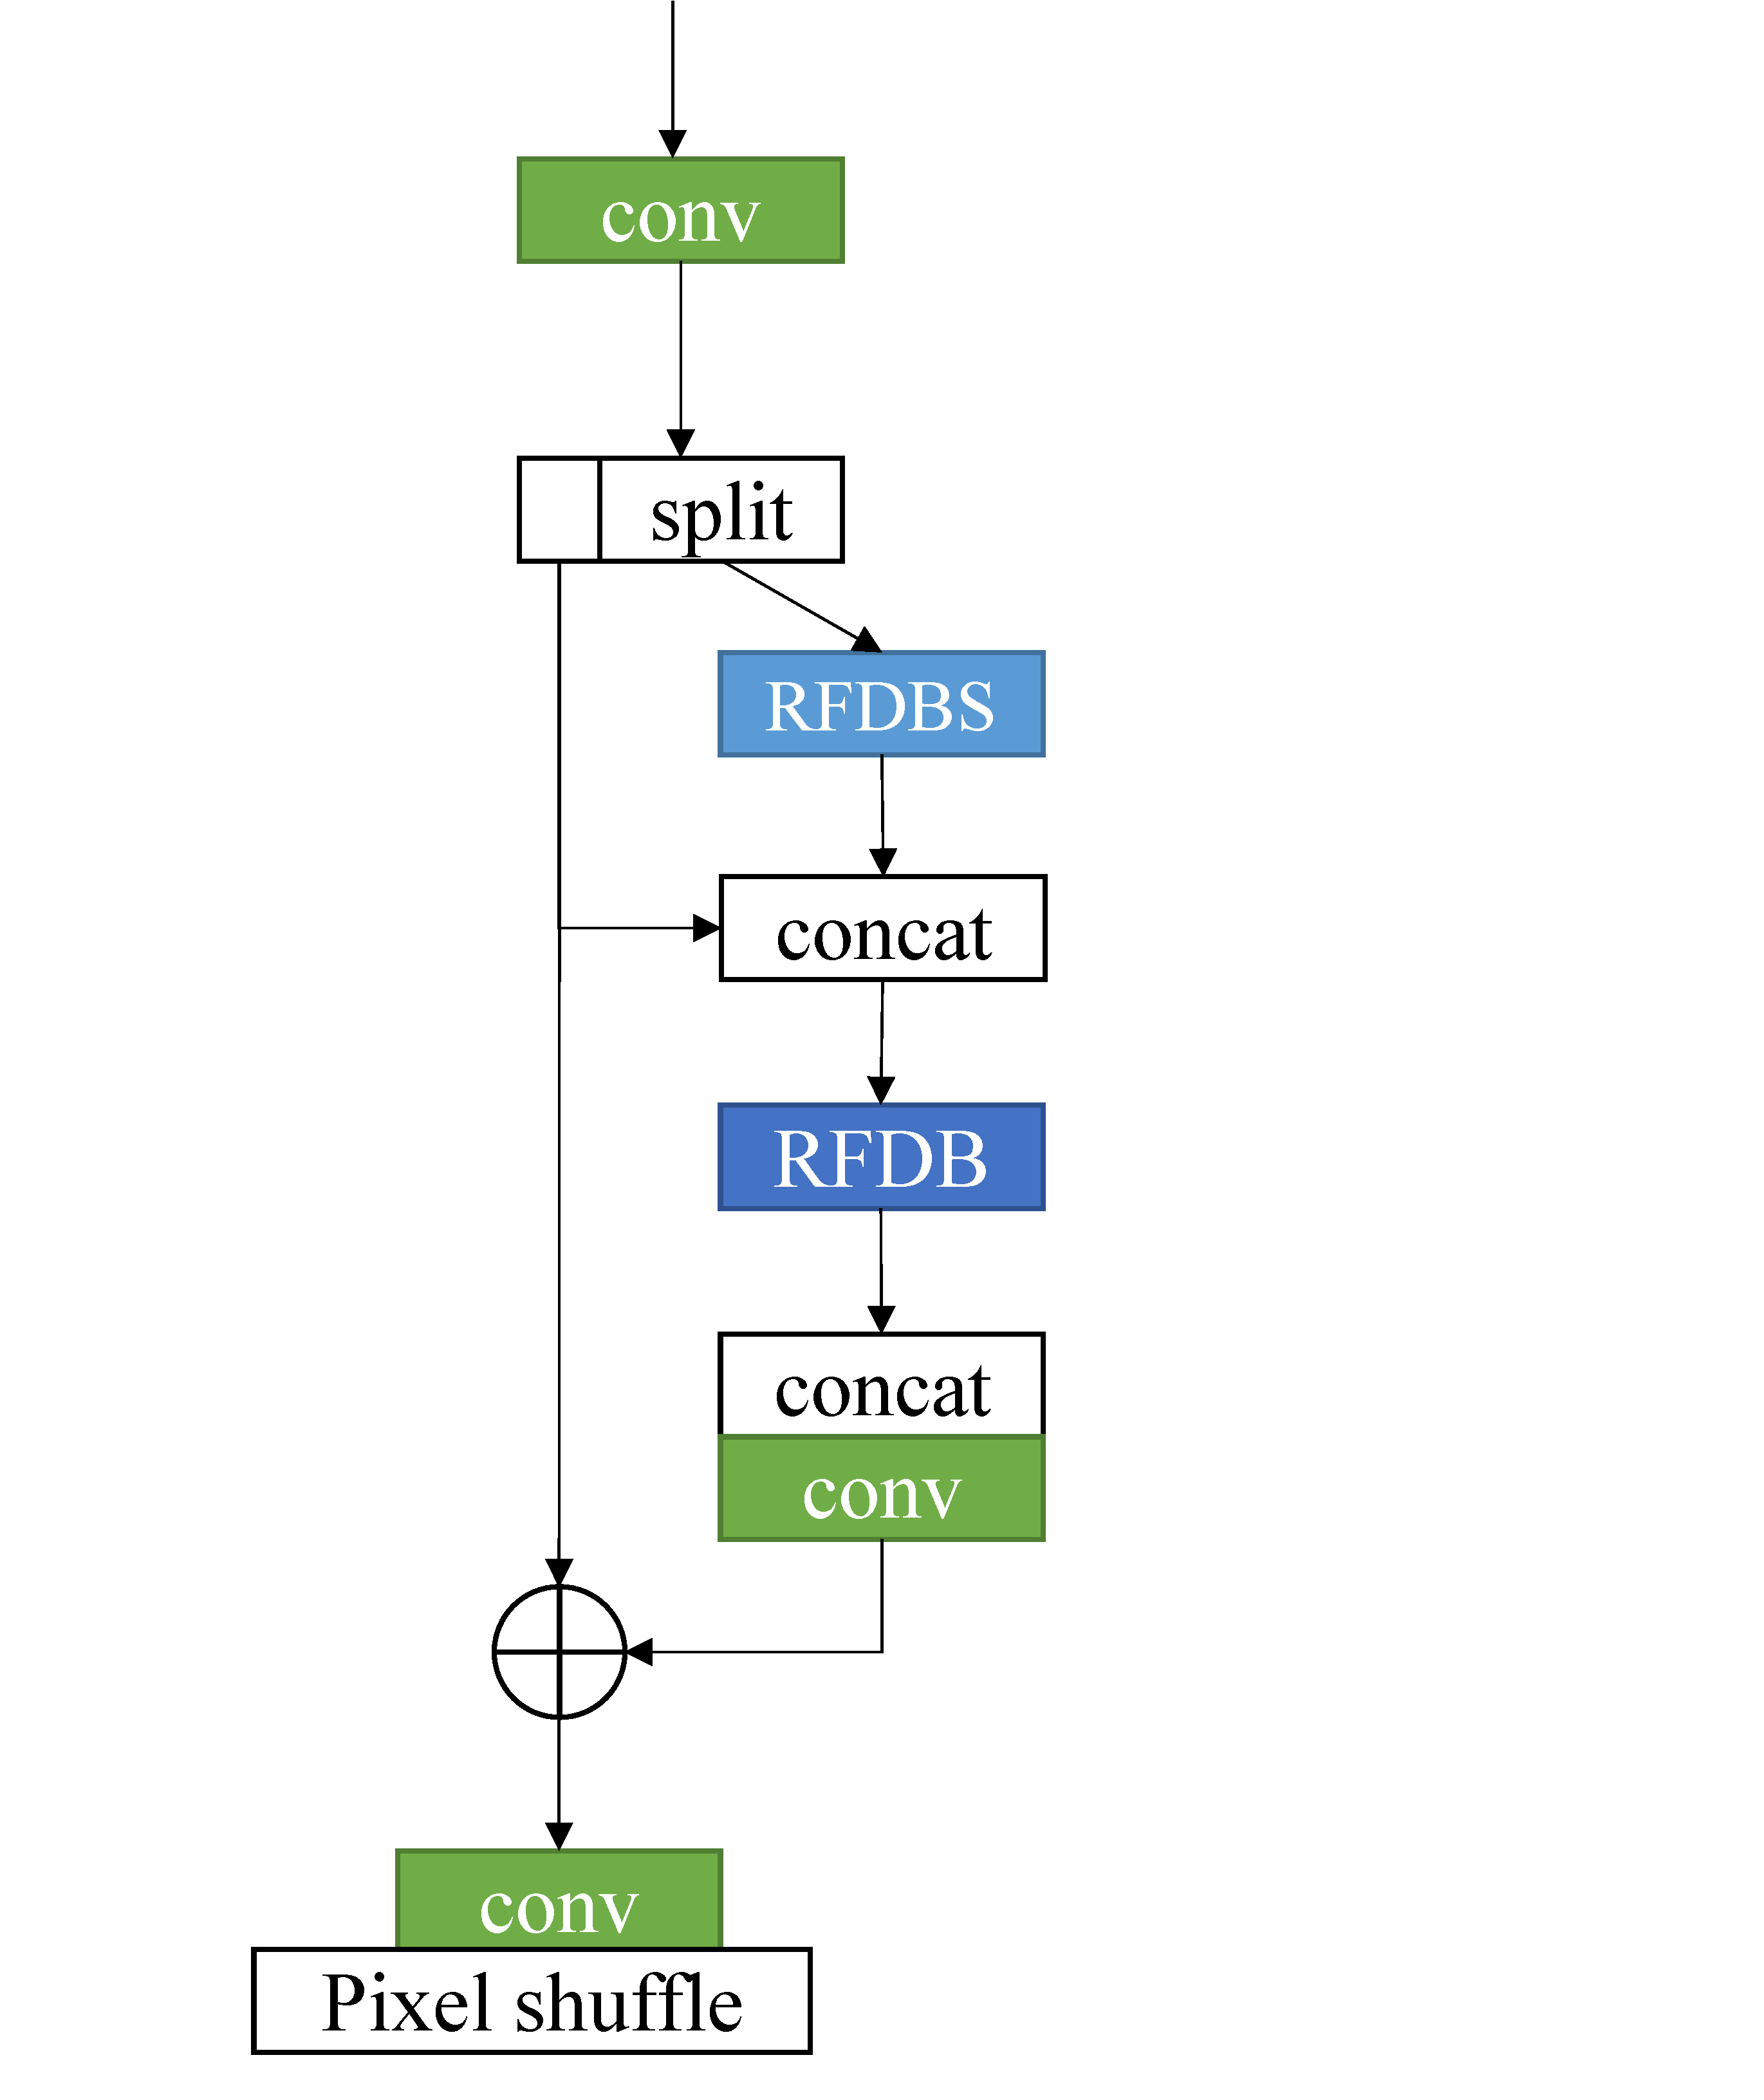
\includegraphics[width=\textwidth]{../Pruning.pdf}
        \caption{Pruning}
        \label{fig:Pruning}
    \end{subfigure}
    \caption{Transform a pre-trained RFDN into PRFDN}
    \label{fig:PRFDN}
\end{figure*}

\noindent
FAQ\medskip\\
{\bf Q:} Are acknowledgements OK?\\
{\bf A:} No.  Leave them for the final copy.\medskip\\
{\bf Q:} How do I cite my results reported in open challenges?
{\bf A:} To conform with the double-blind review policy, you can report results of other challenge participants together with your results in your paper.
For your results, however, you should not identify yourself and should not mention your participation in the challenge.
Instead present your results referring to the method proposed in your paper and draw conclusions based on the experimental comparison to other results.\medskip\\

%-------------------------------------------------------------------------
\subsection{References}

List and number all bibliographical references in 9-point Times, single-spaced, at the end of your paper.
When referenced in the text, enclose the citation number in square brackets, for
example~\cite{Authors14}.
Where appropriate, include page numbers and the name(s) of editors of referenced books.
When you cite multiple papers at once, please make sure that you cite them in numerical order like this \cite{Alpher02,Alpher03,Alpher05,Authors14b,Authors14}.
If you use the template as advised, this will be taken care of automatically.

\begin{table}
  \centering
  \begin{tabular}{@{}lc@{}}
    \toprule
    Method & Frobnability \\
    \midrule
    Theirs & Frumpy \\
    Yours & Frobbly \\
    Ours & Makes one's heart Frob\\
    \bottomrule
  \end{tabular}
  \caption{Results.   Ours is better.}
  \label{tab:example}
\end{table}

%------------------------------------------------------------------------
\section{Final copy}

You must include your signed IEEE copyright release form when you submit your finished paper.
We MUST have this form before your paper can be published in the proceedings.

Please direct any questions to the production editor in charge of these proceedings at the IEEE Computer Society Press:
\url{https://www.computer.org/about/contact}.

\begin{figure*}[t]
    \begin{center}
    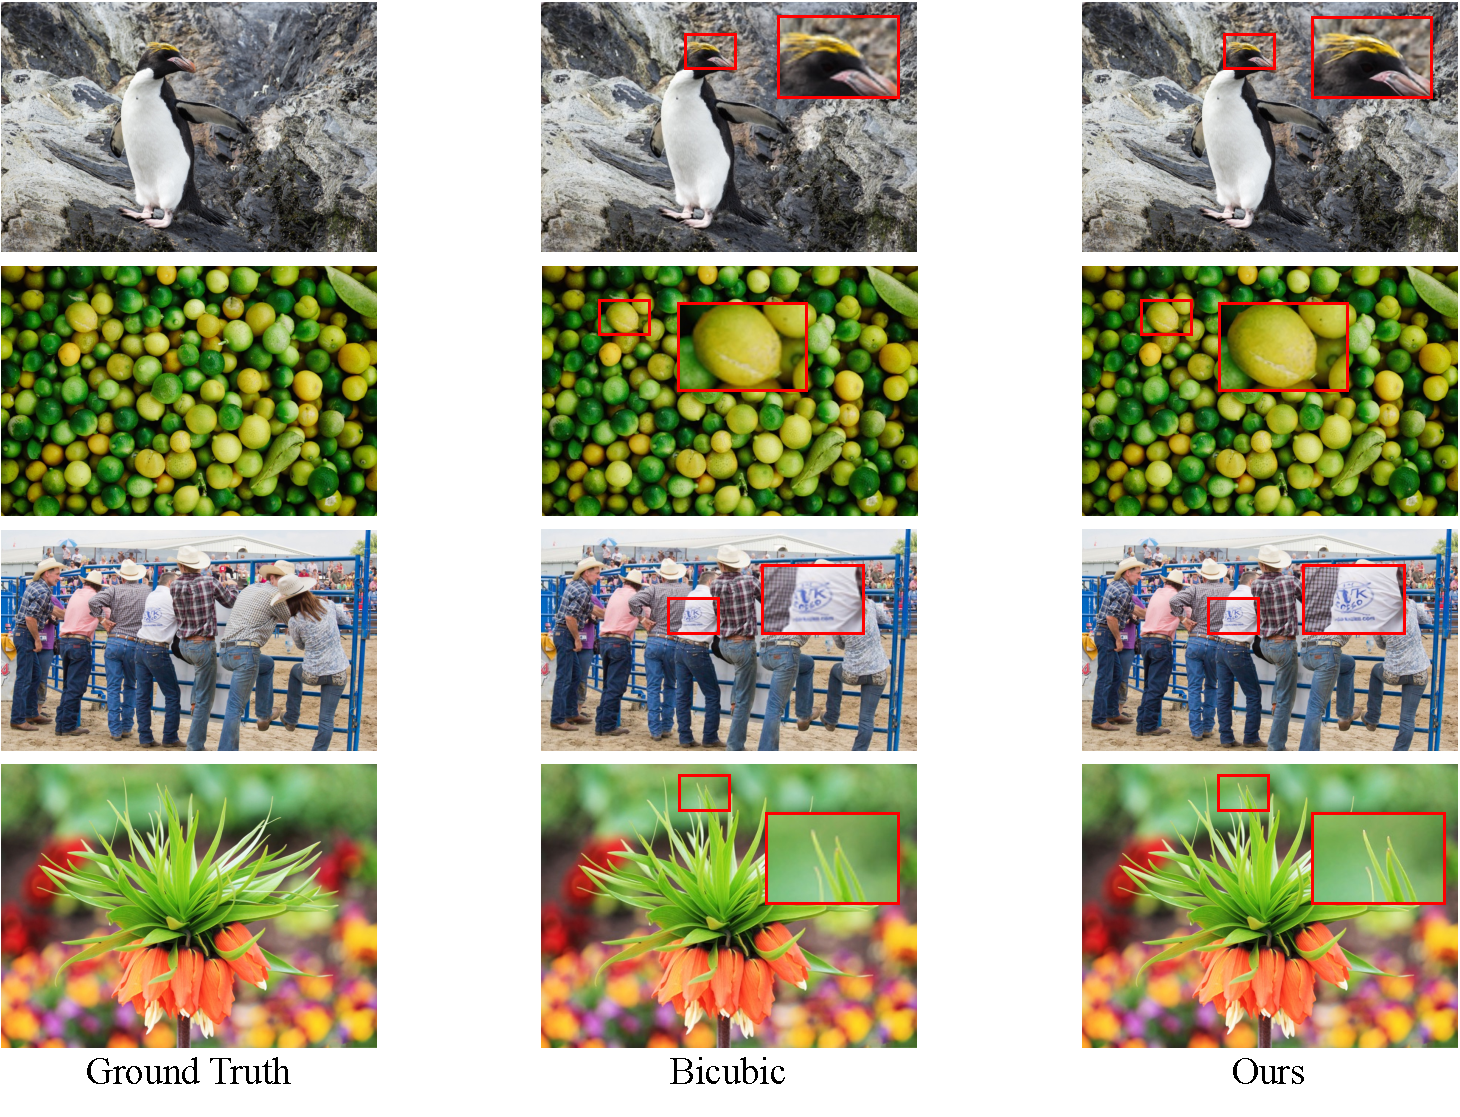
\includegraphics[width=\textwidth]{../x4result.pdf}
    \end{center}
    \caption{Comparison of image quality between our method and the bicubic method.}
    \label{yolov3}
\end{figure*}

\section{Experimental Evaluation}
In this section, we evaluate our our proposed image super-resolution algorithm through various experiments. The experimental setting is first described, including experiment datasets, hardware and software configurations, and assessment measures. Besides, we present the results of our experiments, and compare our method with other existing study to demonstrate the success of our approach.

\subsection{Experimental Setup}

\subsubsection{Datasets}
We used Set5, Set14, BSDS100, and Urban100 datasets to verify the effectiveness of the image recovery quality of our method. These datasets contain a diverse range of images with different levels of complexity, making them suitable for evaluating the performance of super-resolution algorithms.

We evaluated our approach's computational efficiency using some widely used datasets in the field of super-resolution: DIV2K\cite{div2k}, LSDIR\cite{lilsdir}.

The DIV2K dataset is a widely used dataset for super-resolution tasks. It comprises 1000 images characterized by significantly higher resolution than those of the commonly referenced datasets. All the 1000 images are 2K resolution, that is they have 2K pixels on at least one of the axes(vertical or horizontal). All the images were processed using the same tools to $\times2$, $\times3$, and $\times4$ downscaling factors. The images cover a variety of scenes, including landscapes, portraits, and still-life compositions.

The LSDIR dataset proposes a large scale dataset for image restoration. It contains 84,991 high-quality training images and 250 validation images from the whole validation set. The dataset provides both high and low-resolution images for $\times2$, $\times3$, and $\times4$ downscaling factors.

The others 

\subsubsection{Hardware and Software Configurations}
We conducted all experiments on the laptop with an NVIDIA GeForce RTX 3070 GPU, 512GB of RAM, and an Intel(R) Xeon(R) Gold 6230R CPU in the PyTorch environment (version 1.13.0). When training the model, we used the Adam optimizer with a learning rate of 1e-5 and a batch size of 16. We trained the model on the DIV2K dataset for 300 epochs and the LSDIR dataset for 300 epochs.

\subsubsection{Evaluation Metrics}
In the experiment, Peak signal-to-noise ratio (PSNR) and structural similarity index (SSIM), two common evaluation metrics, are used to evalute the performance of our algorithm.  
Additionally, we report the validation time, test time, average time, model parameters, floating-point operations (FLOPs), activation volume, and memory consumption associated with our proposed algorithm. These metrics provide a comprehensive evaluation of effectiveness and computational efficiency about our method.

\subsection{Results}
Our approach has performed well through a series of experiments. The method increases the PSNR and SSIM scores by 10\% and 15\% respectively, compared to the bicubic interpolation algorithm. These results demonstrate the effectiveness of our proposed super-resolution algorithm on high-resolution images. Table \ref{table-time} shows the PSNR and SSIM scores of our method compared to some existing methods on different datasets.

Additionally, our method achieves fast test and validation times, demonstrating its superior computational efficiency. On the DIV2K dataset, Table \ref{table-time} shows the performance of our proposed approach on the DIV2K dataset in terms of validation time, test time, average time, and memory usage compared with state-of-the-art methods. Our method achieves a fast average time with 10000ms on the DIV2K dataset. Both the test time and the validation time are particularly low. Specifically, our approach achieved a low validation time of 10000ms. The memory consumption of our approach is 10000MB.

\begin{table}[h]
  \centering
  \caption{Results.   Ours is better.}
  \resizebox{\linewidth}{!}{
  \begin{tabular}{lccccc}
    \toprule
    Ave Time[ms] & Params[M] &FLOPs[G] &Acts [M] & Mem[M] &Conv\\
    \midrule
    25.97&00.402&25.23&81.88&344.51&39\\
    \bottomrule
  \end{tabular}
  }
  \label{tab:example}
\end{table}

% Table generated by Excel2LaTeX from sheet 'Sheet1'

\begin{table}[htbp]
    \resizebox{\columnwidth}{!}
    {
        \begin{tabular}{|c|c|c|c|c|c|c|c|}
        \hline
        \multirow{2}{*}{Method} & \multirow{2}{*}{Scale} & \multirow{2}{*}{Params} & Set5  & Set14 & BSD100 & Urban100 & Manga109 \bigstrut\\
    \cline{4-8}          &       &       & PSNR/SSIM & PSNR/SSIM & PSNR/SSIM & PSNR/SSIM & PSNR/SSIM \bigstrut\\
        \hline
        Bicubic & \multirow{14}[2]{*}{×2} & -     & 33.66/0.9299 & 30.24/0.8688 & 29.56/0.8431 & 26.88/0.8403 & 30.80/0.9339 \bigstrut[t]\\
        SRCNN[5] &       & 8K    & 36.66/0.9542 & 32.45/0.9067 & 31.36/0.8879 & 29.50/0.8946 & 35.60/0.9663 \\
        FSRCNN[6] &       & 13K   & 37.00/0.9558 & 32.63/0.9088 & 31.53/0.8920 & 29.88/0.9020 & 36.67/0.9710 \\
        VDSR[19][13] &       & 666K  & 37.53/0.9587 & 33.03/0.9124 & 31.90/0.8960 & 30.76/0.9140 & 37.22/0.9750 \\
        DRCN[32][14] &       & 1774K & 37.63/0.9588 & 33.04/0.9118 & 31.85/0.8942 & 30.75/0.9133 & 37.55/0.9732 \\
        DRRN[30] &       & 298K  & 37.74/0.9591 & 33.23/0.9136 & 32.05/0.8973 & 31.23/0.9188 & 37.88/0.9749 \\
        MemNet[35] &       & 678K  & 37.78/0.9597 & 33.28/0.9142 & 32.08/0.8978 & 31.31/0.9195 & 37.72/0.9740 \\
        IDN[12] &       & 553K  & 37.83/0.9600 & 33.30/0.9148 & 32.08/0.8985 & 31.27/0.9196 & 38.01/0.9749 \\
        SRMDNF[42] &       & 1511K & 37.79/0.9601 & 33.32/0.9159 & 32.05/0.8985 & 31.33/0.9204 & 38.07/0.9761 \\
        CARN[1] &       & 1592K & 37.76/0.9590 & 33.52/0.9166 & 32.09/0.8978 & 31.92/0.9256 & 38.36/0.9765 \\
        LAPAR-A[18] &       & 548k  & 38.01/0.9605 & 33.62/0.9183 & 32.19/0.8999 & 32.10/0.9283 & 38.67/0.9772 \\
        IMDN[11] &       & 694K  & 38.00/0.9605 & 33.63/0.9177 & 32.19/0.8996 & 32.17/0.9283 & 38.88/0.9774 \\
        RFDN[24] &       & 534K  & 38.05/0.9606 & 33.68/0.9184 & 32.16/0.8994 & 32.12/0.9278 & 38.88/0.9773 \\
        HNCT (Ours) &       & 356K  & 38.08/0.9608 & 33.65/0.9182 & 32.22/0.9001 & 32.22/0.9294 & 38.87/0.9774 \bigstrut[b]\\
        \hline
        \end{tabular}%
    }
\end{table}%


\subsection{Discussion}
Our super-resoluton algorithm performed well on two challenging datasets with great effectiveness and computational efficiency. On both the DIV2K and LSDIR datasets, our method achieved high PSNR and SSIM scores, indicating that our approach can greatly improve image resolution while preserving image features and textures.

Additionally,when compared to the baseline method, our method demonstrated outstanding computing efficiency, reaching a rapid average time and low memory consumption, which is crucial for real-world applications requiring real-time super-resolution processing, such as video streaming and surveillance.

Although our study achieved encouraging results, some limitations and potential future research approaches should be addressed. We only tested our algorithm on two datasets with a limited number of images, which might be expanded upon in future research.

%%%%%%%%% REFERENCES
{\small
\bibliographystyle{ieee_fullname}
\bibliography{egbib}
}

\end{document}
